% TikZ plot for 2025_dist_shift_2023
% Generated automatically with embedded data
% Requires: \usepackage{pgfplots} \pgfplotsset{compat=1.18}

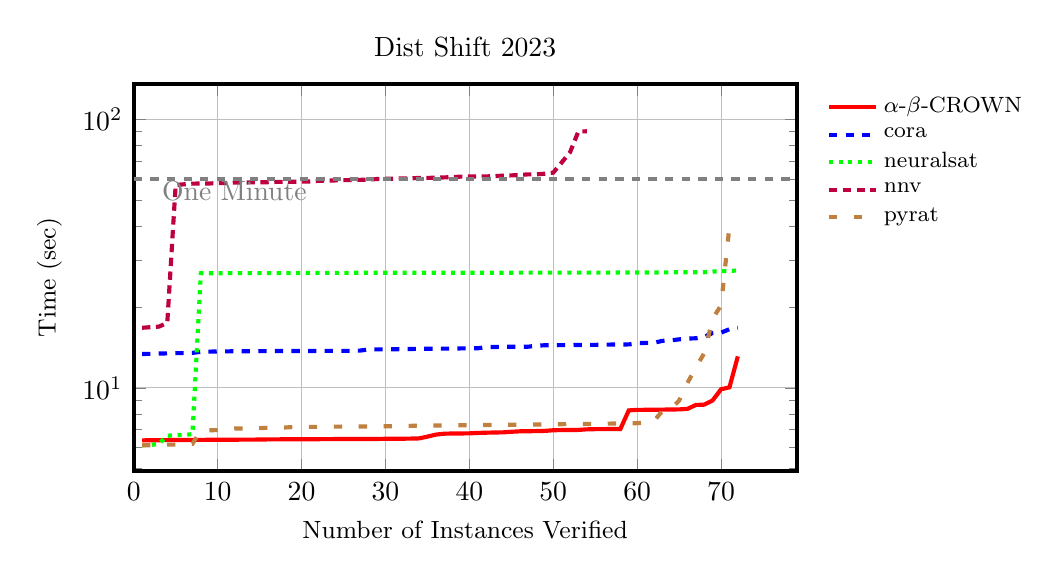
\begin{tikzpicture}
\begin{semilogyaxis}[
    xlabel={Number of Instances Verified},
    ylabel={Time (sec)},
    legend pos=outer north east,
    grid=major,
    width=10cm,
    height=6.5cm,
    ymin=4.891,
    ymax=135.5,
    xmin=0,
    xmax=79,
    line width=1.5pt,
    legend style={font=\footnotesize, cells={anchor=west}, draw=none},
    xlabel style={font=\small},
    ylabel style={font=\small},
    title={Dist Shift 2023},
    title style={font=\normalsize}
]

\addplot[color=red, mark=none, solid] coordinates {
    (1,6.378813)
    (2,6.379120)
    (3,6.381351)
    (4,6.392126)
    (5,6.394921)
    (6,6.399849)
    (7,6.400360)
    (8,6.403166)
    (9,6.408351)
    (10,6.408707)
    (11,6.409368)
    (12,6.410990)
    (13,6.417647)
    (14,6.418085)
    (15,6.421718)
    (16,6.429514)
    (17,6.432217)
    (18,6.435725)
    (19,6.436077)
    (20,6.436670)
    (21,6.437795)
    (22,6.441430)
    (23,6.446210)
    (24,6.447923)
    (25,6.449036)
    (26,6.449702)
    (27,6.451995)
    (28,6.452535)
    (29,6.453214)
    (30,6.464153)
    (31,6.465075)
    (32,6.466429)
    (33,6.474478)
    (34,6.484537)
    (35,6.583381)
    (36,6.698684)
    (37,6.751791)
    (38,6.763960)
    (39,6.766378)
    (40,6.770821)
    (41,6.796328)
    (42,6.810088)
    (43,6.823025)
    (44,6.829625)
    (45,6.863043)
    (46,6.891331)
    (47,6.893971)
    (48,6.907355)
    (49,6.915985)
    (50,6.954973)
    (51,6.965621)
    (52,6.968229)
    (53,6.974605)
    (54,7.009097)
    (55,7.019865)
    (56,7.024267)
    (57,7.027865)
    (58,7.028542)
    (59,8.245521)
    (60,8.281179)
    (61,8.286987)
    (62,8.291041)
    (63,8.300134)
    (64,8.311640)
    (65,8.315748)
    (66,8.355266)
    (67,8.640701)
    (68,8.661118)
    (69,8.985232)
    (70,9.884711)
    (71,10.048276)
    (72,13.102020)
};
\addlegendentry{$\alpha$-$\beta$-CROWN}

\addplot[color=blue, mark=none, dashed] coordinates {
    (1,13.376571)
    (2,13.390532)
    (3,13.429635)
    (4,13.444292)
    (5,13.470843)
    (6,13.481284)
    (7,13.507301)
    (8,13.623572)
    (9,13.646593)
    (10,13.675041)
    (11,13.676206)
    (12,13.693532)
    (13,13.693878)
    (14,13.700113)
    (15,13.704353)
    (16,13.706919)
    (17,13.721815)
    (18,13.722966)
    (19,13.723385)
    (20,13.726382)
    (21,13.727429)
    (22,13.729701)
    (23,13.733177)
    (24,13.733611)
    (25,13.733644)
    (26,13.736690)
    (27,13.773902)
    (28,13.906857)
    (29,13.912791)
    (30,13.925374)
    (31,13.927701)
    (32,13.948080)
    (33,13.962010)
    (34,13.979380)
    (35,13.990775)
    (36,13.999433)
    (37,14.001281)
    (38,14.012221)
    (39,14.031178)
    (40,14.034381)
    (41,14.047392)
    (42,14.184071)
    (43,14.204402)
    (44,14.224354)
    (45,14.225795)
    (46,14.231393)
    (47,14.239145)
    (48,14.356736)
    (49,14.418921)
    (50,14.425540)
    (51,14.426755)
    (52,14.430229)
    (53,14.447152)
    (54,14.456345)
    (55,14.467444)
    (56,14.479931)
    (57,14.505196)
    (58,14.516637)
    (59,14.520374)
    (60,14.674955)
    (61,14.707536)
    (62,14.724861)
    (63,14.968249)
    (64,15.032039)
    (65,15.165343)
    (66,15.264260)
    (67,15.307286)
    (68,15.510290)
    (69,16.021455)
    (70,16.055497)
    (71,16.545611)
    (72,16.722587)
};
\addlegendentry{cora}

\addplot[color=green, mark=none, dotted] coordinates {
    (1,6.114992)
    (2,6.130681)
    (3,6.193266)
    (4,6.634140)
    (5,6.671334)
    (6,6.680170)
    (7,6.726649)
    (8,26.718268)
    (9,26.731113)
    (10,26.735708)
    (11,26.749780)
    (12,26.752017)
    (13,26.752949)
    (14,26.753054)
    (15,26.759859)
    (16,26.763032)
    (17,26.764020)
    (18,26.776581)
    (19,26.789925)
    (20,26.794654)
    (21,26.806219)
    (22,26.808854)
    (23,26.819466)
    (24,26.824655)
    (25,26.828883)
    (26,26.829746)
    (27,26.835317)
    (28,26.839459)
    (29,26.840267)
    (30,26.840551)
    (31,26.842383)
    (32,26.842581)
    (33,26.844660)
    (34,26.847109)
    (35,26.849174)
    (36,26.853827)
    (37,26.854630)
    (38,26.856107)
    (39,26.858739)
    (40,26.858926)
    (41,26.860112)
    (42,26.860362)
    (43,26.861720)
    (44,26.862504)
    (45,26.863566)
    (46,26.866698)
    (47,26.869908)
    (48,26.870300)
    (49,26.872038)
    (50,26.875749)
    (51,26.876960)
    (52,26.878615)
    (53,26.885183)
    (54,26.886218)
    (55,26.886477)
    (56,26.886481)
    (57,26.889623)
    (58,26.890179)
    (59,26.891988)
    (60,26.898499)
    (61,26.917234)
    (62,26.919899)
    (63,26.925829)
    (64,26.945050)
    (65,26.948390)
    (66,26.958833)
    (67,26.960763)
    (68,26.974024)
    (69,27.134190)
    (70,27.209096)
    (71,27.265563)
    (72,27.391273)
};
\addlegendentry{neuralsat}

\addplot[color=purple, mark=none, densely dashed] coordinates {
    (1,16.746201)
    (2,16.835967)
    (3,16.914859)
    (4,17.464106)
    (5,57.029193)
    (6,57.325934)
    (7,57.664902)
    (8,57.718568)
    (9,57.732469)
    (10,57.936051)
    (11,57.950083)
    (12,58.175023)
    (13,58.214445)
    (14,58.286307)
    (15,58.307505)
    (16,58.384218)
    (17,58.524138)
    (18,58.556265)
    (19,58.592338)
    (20,58.691459)
    (21,58.733135)
    (22,59.060116)
    (23,59.193168)
    (24,59.264473)
    (25,59.406949)
    (26,59.468686)
    (27,59.562182)
    (28,59.711594)
    (29,59.988912)
    (30,60.090435)
    (31,60.166205)
    (32,60.295166)
    (33,60.328260)
    (34,60.555106)
    (35,60.562098)
    (36,60.674230)
    (37,60.830542)
    (38,60.959157)
    (39,61.246366)
    (40,61.302873)
    (41,61.322365)
    (42,61.352286)
    (43,61.479288)
    (44,61.732653)
    (45,61.886676)
    (46,62.101739)
    (47,62.423934)
    (48,62.449965)
    (49,62.788925)
    (50,63.361263)
    (51,69.093639)
    (52,75.456308)
    (53,90.241975)
    (54,90.310845)
};
\addlegendentry{nnv}

\addplot[color=brown, mark=none, loosely dashed] coordinates {
    (1,6.113308)
    (2,6.117303)
    (3,6.124117)
    (4,6.147198)
    (5,6.149200)
    (6,6.156018)
    (7,6.192330)
    (8,6.944579)
    (9,6.957433)
    (10,6.960470)
    (11,7.006204)
    (12,7.058093)
    (13,7.058699)
    (14,7.081333)
    (15,7.082213)
    (16,7.104667)
    (17,7.119087)
    (18,7.121317)
    (19,7.148679)
    (20,7.152787)
    (21,7.157929)
    (22,7.160730)
    (23,7.165765)
    (24,7.173234)
    (25,7.178301)
    (26,7.178934)
    (27,7.179012)
    (28,7.179472)
    (29,7.198017)
    (30,7.198242)
    (31,7.201561)
    (32,7.217515)
    (33,7.221828)
    (34,7.238782)
    (35,7.242751)
    (36,7.244312)
    (37,7.250720)
    (38,7.257777)
    (39,7.263008)
    (40,7.264843)
    (41,7.273801)
    (42,7.278908)
    (43,7.281298)
    (44,7.285865)
    (45,7.290239)
    (46,7.291342)
    (47,7.292788)
    (48,7.309608)
    (49,7.310405)
    (50,7.311441)
    (51,7.326183)
    (52,7.330337)
    (53,7.333542)
    (54,7.335029)
    (55,7.347816)
    (56,7.350525)
    (57,7.366098)
    (58,7.369336)
    (59,7.370773)
    (60,7.391893)
    (61,7.427618)
    (62,7.528114)
    (63,8.200794)
    (64,8.340701)
    (65,8.968883)
    (66,10.433622)
    (67,11.955776)
    (68,13.462716)
    (69,18.137638)
    (70,20.292318)
    (71,39.998028)
};
\addlegendentry{pyrat}

% Timeout line
\addplot[color=gray, dashed, mark=none, domain=0:79] {60};

% Add timeout label as text below the line
\node[color=gray] at (axis cs:12,54.0) {One Minute};

\end{semilogyaxis}
\end{tikzpicture}
